\documentclass{exam}
\usepackage[a4paper, margin=2cm]{geometry}
\usepackage{graphicx}
\usepackage{amsmath}
\usepackage{amssymb}

\printanswers

% Define the \coursegroup command
\newcommand{\coursegroup}{A}

% Footer customization using exam class commands
\footer{}{BLM2011 Statistics and Probability Calculations, Final Exam, Gr 1, Key \coursegroup, Page \thepage}{}

\begin{document}

\begin{center}
    \fbox{\fbox{\parbox{5.5in}{\centering
    BLM2011	Statistics and Probability Calculations Final Exam\\
    2023 - 2024 Fall, 9 Jan 2024, Key \coursegroup}}}
\end{center}



\noindent % No indentation at the beginning of the paragraph
\begin{minipage}{0.5\textwidth} % Adjust the width of the minipage as needed
    \fbox{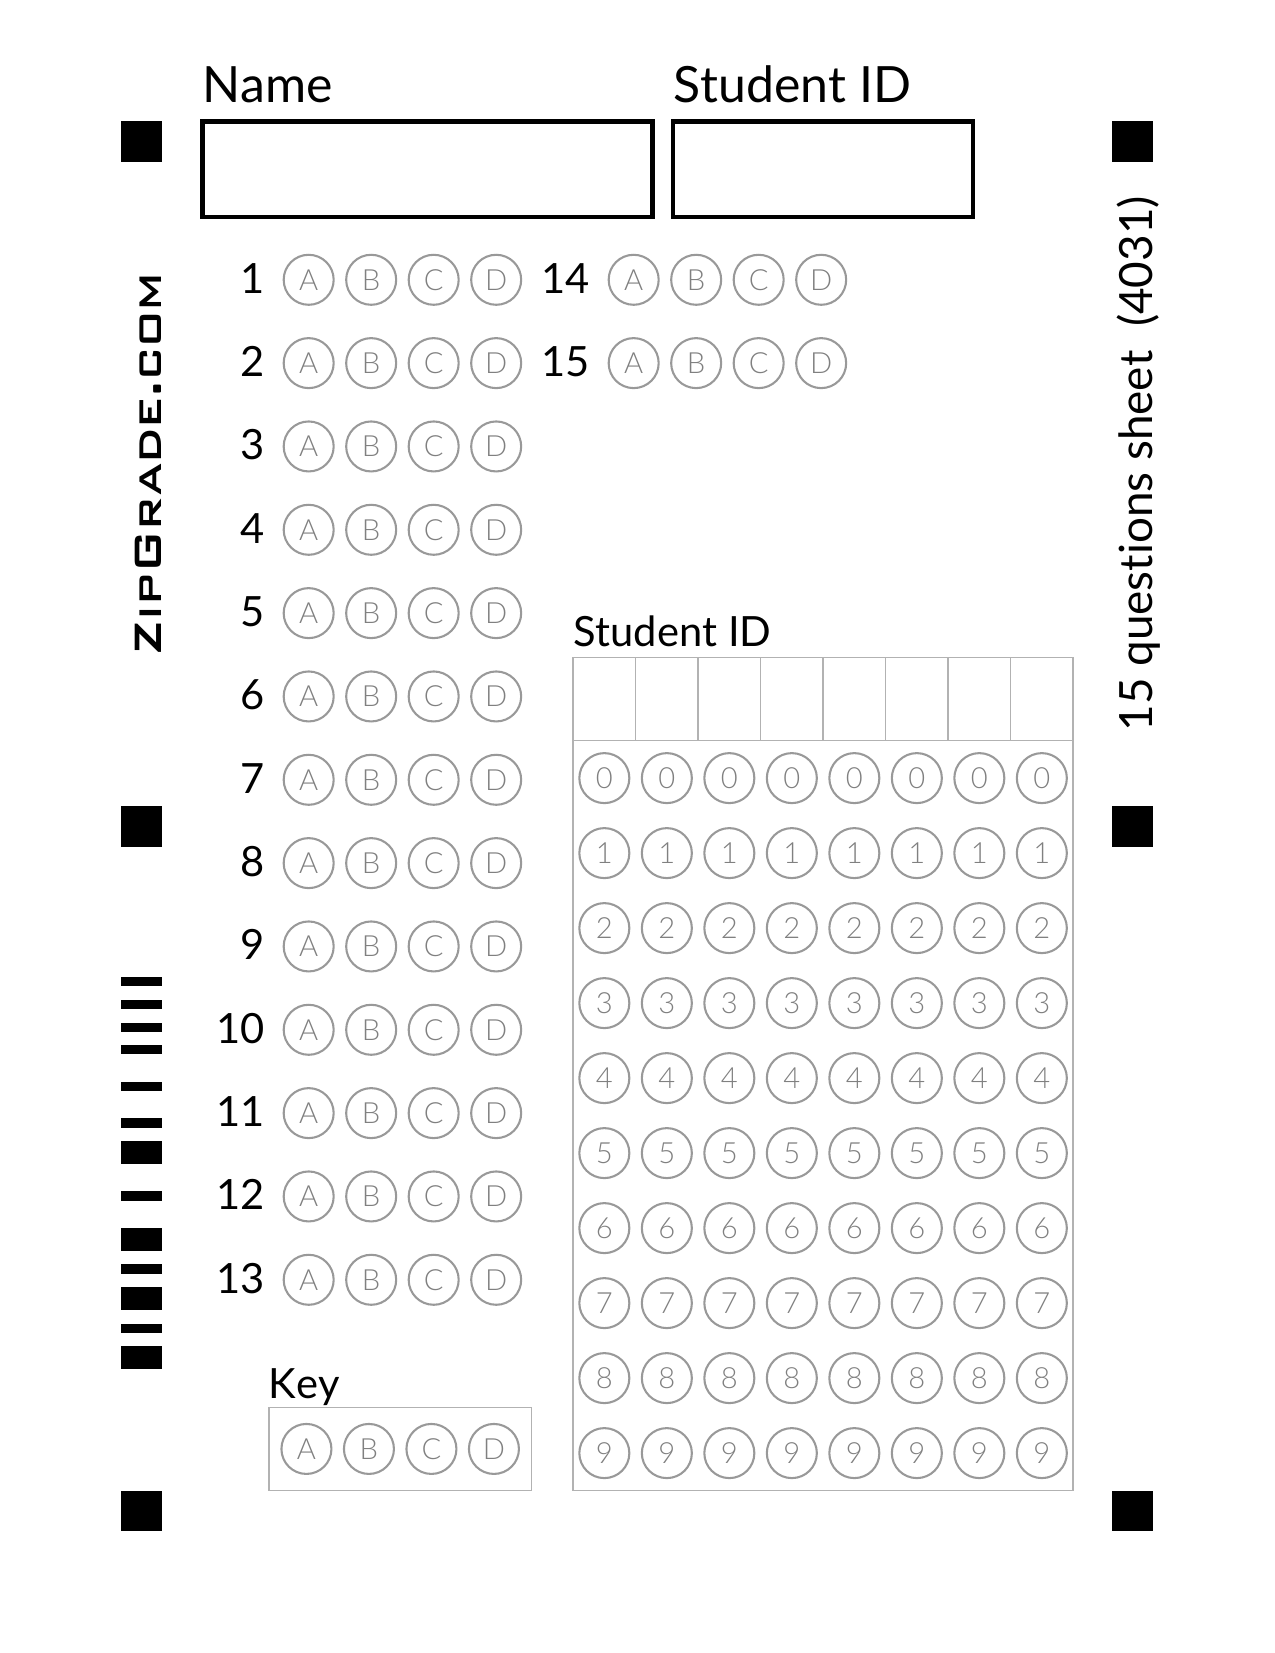
\includegraphics[width=0.9\linewidth]{4031.png}}
\end{minipage}%
\hfill% Fill the horizontal space to push the next minipage to the right
\begin{minipage}{0.4\textwidth} % Adjust the width of the minipage as needed
    \textbf{Notes to exam supervisors}: 
        * Exam duration is 110 minutes. * Do not allow students out first 30 minutes, and accept new students only first 30 minutes. * Check each student to see they filled answer sheet name, student id, and key correctly. * Students can use calculators. They can have a scrap paper to write on. Gather the scrap papers at the end of the exam. * Separate student papers into keys at the end of the exam. Gather scrap papers separately, do not interleave to student papers.
        
    \textbf{Notes to students}: 
        * Please enter your name and student ID in the provided spaces and indicate your student ID by filling in the corresponding bubbles. * Enter your answers to the answer sheet. The exam will be graded optically. * Make sure you fill the correct "Key" bubble. * If you think a question may be wrong, tell to the exam supervisors. They will inform me. 
        
        * Standard Normal Distribution Cumulative Distribution Values: 
    
        $\Phi(-1)\approx 0.16$, $\Phi(1)\approx 0.84$, $\Phi(2.24)\approx 0.98$,  $\Phi(2.18)=0.9854$, $\Phi(2.29)=0.9890$

        * Standard Normal Distribution Quantiles:
    
        \(z_{0.10} = \Phi^{-1}(0.90) = 1.282\), \(z_{0.05} = 1.645\), \(z_{0.025} = 1.960\), \(z_{0.01} = 2.326\), \(z_{0.005} = 2.576\).


\end{minipage}





\textbf{Questions} (Each equal in points):
\begin{questions}





\question A company offers a referral bonus program. For each referred employee who stays at least 6 months, the referrer gets 500 dollars. If the probability that a referred employee stays for 6 months is 0.4, what is the expected bonus for referring one employee in dollars?

\begin{oneparchoices}
\correctchoice 200
\choice 500
\choice 100
\choice 0
\end{oneparchoices}

\begin{solution}
The expected bonus is \(E(X) = 0.4 \times 500 = 200\) dollars.
\end{solution}
    




\question A basketball player has a 70 percent chance of making each free throw. If she takes 10 free throws, what is the expected number of free throws she will make?

\begin{oneparchoices}
\correctchoice $7$ free throws
\choice $3$ free throws
\choice $10$ free throws
\choice $5$ free throws
\end{oneparchoices}

\begin{solution}
The expected number is \(E(X) = np = 10 \times 0.7 = 7\) free throws.
\end{solution}
    




\question A taxi company charges a flat rate of 3 dollars plus 2 dollars per mile. If the distance of a ride follows a uniform distribution between 1 and 5 miles, what is the expected cost of a ride in dollars?

\begin{oneparchoices}
\correctchoice 9
\choice 8
\choice 10
\choice 7
\end{oneparchoices}

\begin{solution}
The expected distance is the mean of the uniform distribution, \(\frac{1 + 5}{2} = 3\) miles. Thus, the expected cost is \(3 + 2 \times 3 = 9\) dollars.
\end{solution}
    



\end{questions}


\end{document}

